

\tikzset{every picture/.style={line width=0.75pt}} %set default line width to 0.75pt

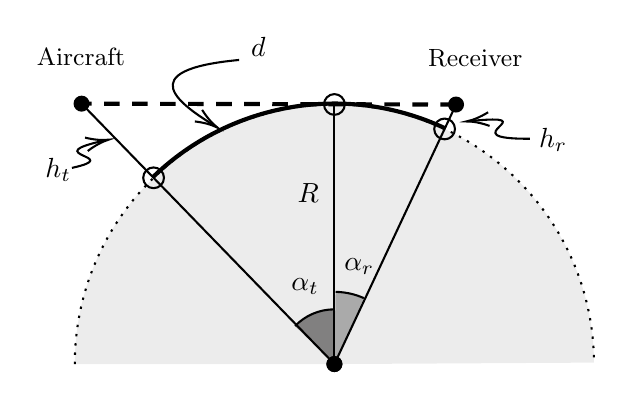
\begin{tikzpicture}[x=0.75pt,y=0.75pt,yscale=-1,xscale=1]
%uncomment if require: \path (0,447); %set diagram left start at 0, and has height of 447

%Shape: Arc [id:dp5690903281113118]
\draw  [draw opacity=0][fill={rgb, 255:red, 236; green, 236; blue, 236 }  ,fill opacity=1 ][dash pattern={on 0.84pt off 2.51pt}] (110.04,201) .. controls (110.04,201) and (110.04,201) .. (110.04,201) .. controls (110.04,131.93) and (166.04,75.93) .. (235.12,75.93) .. controls (303.96,75.93) and (359.82,131.55) .. (360.19,200.3) -- (235.12,201) -- cycle ; \draw  [dash pattern={on 0.84pt off 2.51pt}] (110.04,201) .. controls (110.04,201) and (110.04,201) .. (110.04,201) .. controls (110.04,131.93) and (166.04,75.93) .. (235.12,75.93) .. controls (303.96,75.93) and (359.82,131.55) .. (360.19,200.3) ;
%Straight Lines [id:da3652394426894523]
\draw [line width=1.5]  [dash pattern={on 5.63pt off 4.5pt}]  (293.72,75.96) -- (113.31,75.53) ;


%Curve Lines [id:da0314547922320223]
\draw    (329.24,92.44) .. controls (289.34,92.62) and (339.2,80.05) .. (300.48,83.92) ;
\draw [shift={(298.65,84.11)}, rotate = 353.97] [color={rgb, 255:red, 0; green, 0; blue, 0 }  ][line width=0.75]    (10.93,-3.29) .. controls (6.95,-1.4) and (3.31,-0.3) .. (0,0) .. controls (3.31,0.3) and (6.95,1.4) .. (10.93,3.29)   ;

%Curve Lines [id:da8824974860724117]
\draw    (108.67,106.48) .. controls (134.99,100.68) and (90.76,100.58) .. (124.73,93.23) ;
\draw [shift={(126.33,92.89)}, rotate = 528.24] [color={rgb, 255:red, 0; green, 0; blue, 0 }  ][line width=0.75]    (10.93,-3.29) .. controls (6.95,-1.4) and (3.31,-0.3) .. (0,0) .. controls (3.31,0.3) and (6.95,1.4) .. (10.93,3.29)   ;

%Shape: Arc [id:dp3560200749347655]
\draw  [draw opacity=0][line width=1.5]  (147.84,110.79) .. controls (184.2,75.63) and (239.86,64.64) .. (288.37,87.37) .. controls (288.48,87.42) and (288.58,87.47) .. (288.69,87.52) -- (235.12,201) -- cycle ; \draw  [line width=1.5]  (147.84,110.79) .. controls (184.2,75.63) and (239.86,64.64) .. (288.37,87.37) .. controls (288.48,87.42) and (288.58,87.47) .. (288.69,87.52) ;
%Curve Lines [id:da23413477884430978]
\draw    (189.2,54.48) .. controls (136.23,59.41) and (161.51,76.18) .. (177.22,86.1) ;
\draw [shift={(178.89,87.15)}, rotate = 212.24] [color={rgb, 255:red, 0; green, 0; blue, 0 }  ][line width=0.75]    (10.93,-3.29) .. controls (6.95,-1.4) and (3.31,-0.3) .. (0,0) .. controls (3.31,0.3) and (6.95,1.4) .. (10.93,3.29)   ;

%Shape: Arc [id:dp32891412685871013]
\draw  [draw opacity=0][fill={rgb, 255:red, 170; green, 170; blue, 170 }  ,fill opacity=1 ] (235.67,166.21) .. controls (240.53,166.29) and (245.15,167.36) .. (249.33,169.23) -- (235.12,201) -- cycle ; \draw   (235.67,166.21) .. controls (240.53,166.29) and (245.15,167.36) .. (249.33,169.23) ;
%Shape: Arc [id:dp7029066137990934]
\draw  [draw opacity=0][fill={rgb, 255:red, 129; green, 128; blue, 128 }  ,fill opacity=1 ] (216.18,182.64) .. controls (220.99,177.68) and (227.73,174.61) .. (235.17,174.63) -- (235.12,201) -- cycle ; \draw   (216.18,182.64) .. controls (220.99,177.68) and (227.73,174.61) .. (235.17,174.63) ;
%Straight Lines [id:da8761528166800212]
\draw    (293.72,75.96) -- (235.12,201) ;
\draw [shift={(235.12,201)}, rotate = 115.11] [color={rgb, 255:red, 0; green, 0; blue, 0 }  ][fill={rgb, 255:red, 0; green, 0; blue, 0 }  ][line width=0.75]      (0, 0) circle [x radius= 3.35, y radius= 3.35]   ;
\draw [shift={(293.72,75.96)}, rotate = 115.11] [color={rgb, 255:red, 0; green, 0; blue, 0 }  ][fill={rgb, 255:red, 0; green, 0; blue, 0 }  ][line width=0.75]      (0, 0) circle [x radius= 3.35, y radius= 3.35]   ;
%Straight Lines [id:da6955293230830237]
\draw    (235.12,75.53) -- (235.12,201) ;
\draw [shift={(235.12,201)}, rotate = 90] [color={rgb, 255:red, 0; green, 0; blue, 0 }  ][fill={rgb, 255:red, 0; green, 0; blue, 0 }  ][line width=0.75]      (0, 0) circle [x radius= 3.35, y radius= 3.35]   ;

%Straight Lines [id:da17629850181731288]
\draw    (235.12,201) -- (113.31,75.53) ;
\draw [shift={(113.31,75.53)}, rotate = 225.85] [color={rgb, 255:red, 0; green, 0; blue, 0 }  ][fill={rgb, 255:red, 0; green, 0; blue, 0 }  ][line width=0.75]      (0, 0) circle [x radius= 3.35, y radius= 3.35]   ;


% Text Node
\draw (102.11,107.26) node   [align=left] {$\displaystyle h_{t}$};
% Text Node
\draw (340.5,93.15) node   [align=left] {$\displaystyle h_{r}$};
% Text Node
\draw (222.56,118.43) node   [align=left] {$\displaystyle R$};
% Text Node
\draw (198.49,48) node   [align=left] {$\displaystyle d$};
% Text Node
\draw (113.05,53.17) node  [font=\small] [align=left] {Aircraft};
% Text Node
\draw (302.94,53.49) node  [font=\small] [align=left] {Receiver};
% Text Node
\draw (221,163.55) node   [align=left] {$\displaystyle \alpha _{t}$};
% Text Node
\draw (247.09,154.11) node   [align=left] {$\displaystyle \alpha _{r}$};

\draw   (288.21, 87.72) circle [x radius= 5, y radius= 5]   ;
\draw   (235.12, 75.93) circle [x radius= 5, y radius= 5]   ;
\draw   (148, 111.26) circle [x radius= 5, y radius= 5]   ;
\end{tikzpicture}
